\chapter{Synthèse hybride d'un son de guitare}
\section{Synthèse FRF}

\subsection{Principe}
% méthode hybride ici. mélange mesures et théorie
\paragraph*{} 

Le principe de la synthèse dans le domaine fréquentiel est relativement simple.
Il s'agit de calculer ou de mesurer des fonctions de transfert
(\textit{Frequency Response Function}) nous permettant de relier une force
appliquée au point d'excitation de la corde à un déplacement au niveau du
chevalet, de la table d'harmonie de la guitare, ou d'un autre instrument comme
le ukulélé. Le premier élément nécessaire est l'admittance au chevalet, qui
peut s'exprimer grâce à l'admittance des cordes et celle du corps au niveau du
chevalet (par corps, il faut comprendre la table d'harmonie et la caisse de la
guitare), par l'équation \ref{eq:eq_frf_1}.

\begin{equation}
  \frac{1}{Y_{total}} = \frac{1}{Y_{corps}} + \frac{1}{Y_{corde}}
  \label{eq:eq_frf_1}
\end{equation}

Cette admittance totale au niveau du chevalet nous fournit la vitesse de
celui-ci en fonction d'une force qui y serait appliquée. \\

Le second élément nécessaire est la fonction de transfert $H$ reliant un
déplacement de la corde à un déplacement au niveau du chevalet. En multipliant
cette fonction avec $Y_{total}$, on obtient la FRF fournissant le déplacement
$\delta_{excitation}$ en fonction de la force $F_{chevalet}$. Le système étant
supposé linéaire, cette fonction de transfert fournit aussi le déplacement
$\delta_{chevalet}$ en fonction de la force $F_{excitation}$ :

\begin{equation}
  \frac{\delta_{chevalet}}{F_{excitation}} = \frac{\delta_{excitation}}{F_{chevalet}} = \frac{Y_{total}H}({j\omega})^2
  \label{eq:eq_frf_2}
\end{equation}

\subsection{Mise en place}
% implémentation
% H, Z, Ytotal

L'article de Woodhouse à notre disposition nous a permis d'écrire l'impédance
de la corde au chevalet $Z_{corde}$, ainsi que la fonction de transfert
unitaire $H$ à partir de la connaissance des caractéristiques de la corde :
masse linéique, tension, coefficients d'amortissement, raideur de flexion. Les
mesures sur les instruments nous ont fourni une estimation de $Y_{corps}$ et de
$Y_{total}$. \\

La première approche a été d'utiliser uniquement $Y_{total}$ mesurée en
excitant au marteau d'impact un point proche du chevalet et en mesurant son
accélération selon l'axe normal et l'axe transverse par rapport à la table
d'harmonie. La corde que l'on souhaitait synthétiser était libre de vibrer
alors que les autres étaient étouffées. En réalité, nous mesurions l'inertance,
ce qui devait ajouter une seconde intégration à l'équation \ref{eq:eq_frf_2}.\\

La seconde approche a été de n'utiliser que la mesure de $Y_{corps}$ .
L'admittance de la corde au chevalet a utilisé les formulations théoriques de
l'article. \\

Les FRF issues des mesures temporelles ont été calculées avec un très grand
nombre de point pour que le signal final dure plusieurs secondes.\\

L'obtention du son était en effet réalisée par FFT inverse, ce qui nous a
imposé d'écrire la symétrie hermitienne pour notre fonction de transfert.
L'intégration de l'équation \ref{eq:eq_frf_2} a été omise dans un premier temps
: les valeurs sont divergentes en zéro. Pour compenser cela nous divisions
l'admittance de mesure par 100 ou 1000.\\

Enfin, nous convoluons ce signal avec plusieurs impulsions consécutives pour
adoucir le son et modéliser un plectre basiquement. La force excitatrice n'est
pas un dirac mais $1$ sur $100$ échantillons avant de passer à 0.

\subsection{Résultats}
%
Plusieurs précisions ont du être apportés pour améliorer l'algorithme et le
son. En effet, ce système comporte plusieurs limitations : l'admittance
$Y_{corps}$ est affectée par la présence de cordes même atténuées. Cet effet
est difficilement écarté puisqu'oter les cordes modifie la masse au niveau du
chevalet. Aussi, nous n'avons pas mesuré les caractéristiques des cordes de la
guitare à notre disposition mais nous somnes basés sur des valeurs fournies par
Woodhouse, qui peuvent ne pas correspondre à notre instrument.  \\

Utiliser $Y_{total}$ n'a pas fournit de résultats convaincants. Les sons
synthétisés ne correspondaient pas à ceux d'une guitare. Woodhouse suggère en
effet d'effectuer la séparation de cette grandeur, ce que nous avons fait
ensuite.\\

La figure suivante présente les différentes étapes nous ayant permis de
synthétiser les sons

\begin{figure}[h]
\centering
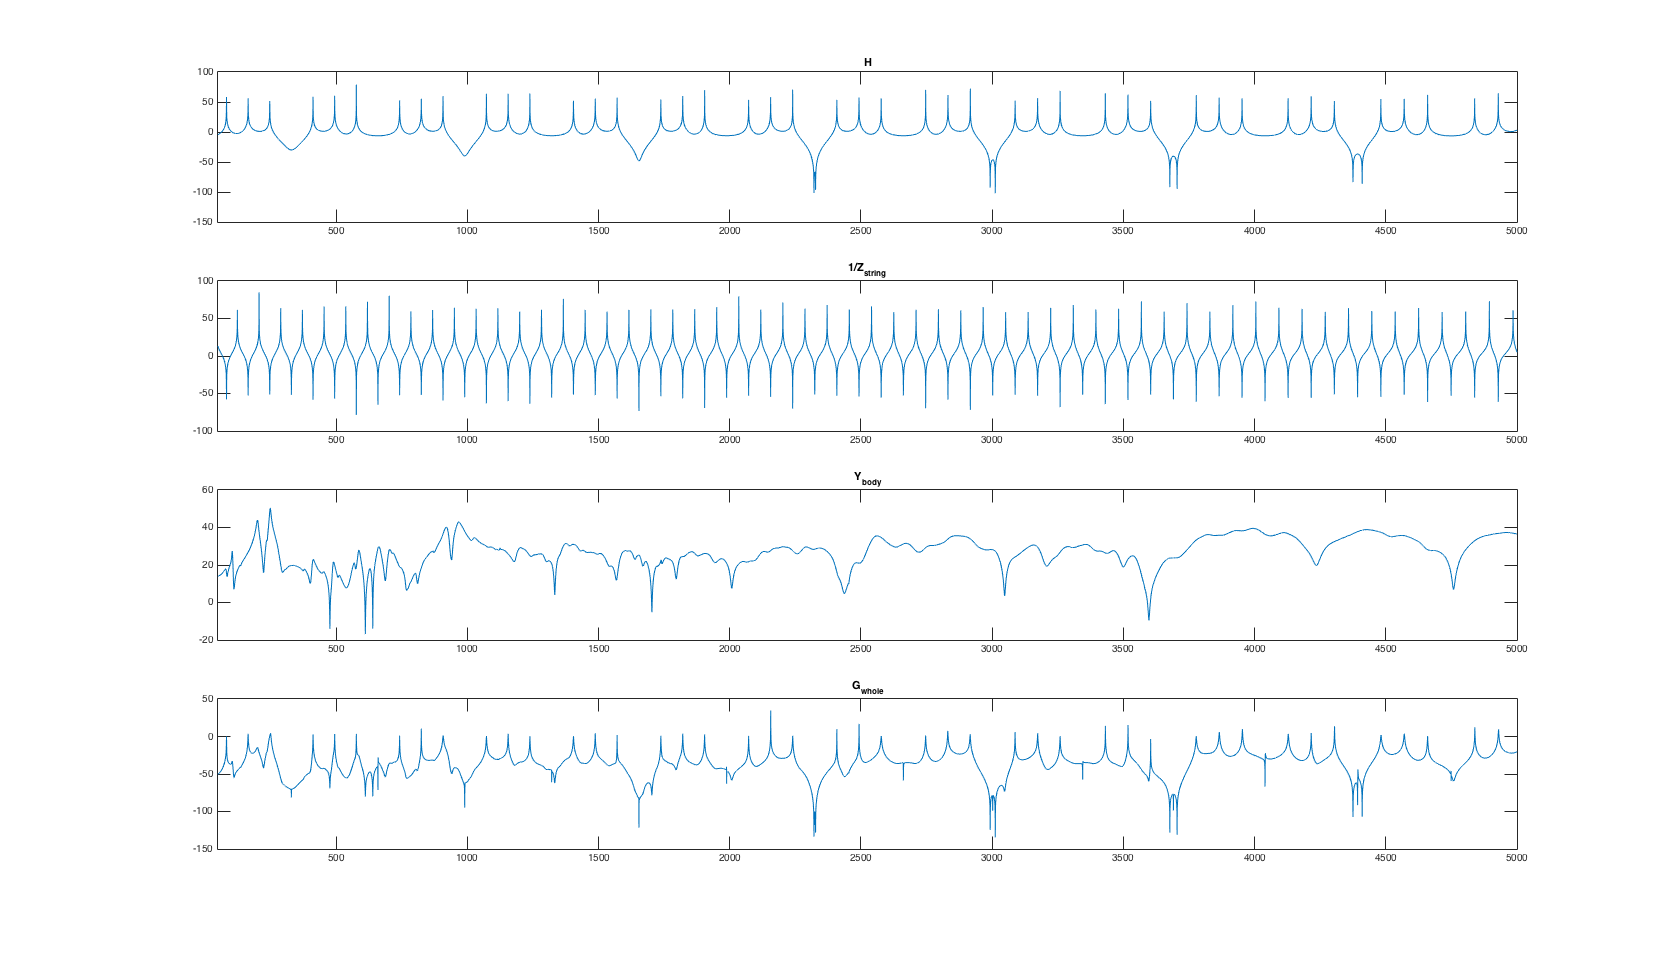
\includegraphics[width=\linewidth]{figures/frf_rapport_intermediaire.png}
\caption{Etapes de calcul de la synthèse FRF}
\label{fig:FRF1}
\end{figure}

La seconde approche a permis d'avoir un son accordé sur la note désirée et de
reconnaître un son de guitare. Cependant il doit encore être précisé car il est
saturé et comporte des fréquences assez élevées avec des atténuations peu
faibles.


%
%
% $c$ pour chevalet, $e$ pour excitation.
% $$\frac{1}{Y_{tot}} = \frac{1}{Y_{corps}} + \frac{1}{Y_{corde}}$$
%$$F_c \times Y_{tot} = v_c$$
%$$v_c \times \tilde{H} = v_e$$
%$$\frac{v_e}{j\omega} = \delta_e$$
%par théorème de réciprocité de Betty : 
%$$\frac{\delta_c}{F_e} = \frac{\delta_e}{F_c} = \frac{Y_{tot}\tilde{H}}{j\omega}$$
%
%


\section{Synthèse modale}

\paragraph{}
  On présente dans cette partie le processus d'analyse/synthèse modale hybride
appliqué dans le cadre du projet. Ce processus est basé sur les principes
suivants : les paramètres physiques découplés de corde et de guitare sont
posés, pour la corde via un modèle théorique, pour le corps en appliquant
\textsc{esprit} sur les mesures d'admittance effectuées et en remontant aux
paramètres physiques du système.
  Ensuite, le système d'équations différentielles à \( N \) modes du système
couplé est posé et on résout ce système pour en extraire les déformées modales
et les fréquences propres du système couplé. Enfin, en posant fixant des
conditions initiales, on peut resynthétiser le son de la corde couplée au
chevalet.

\subsection{Paramètres physiques}

\paragraph{}
Par souci de concision, on ne présente pas dans ce rapport le détail des
matrices développées dans l'article de Woodhouse, mais seulement la façon dont
les paramètres physiques pertinents sont extraits ou fixés.

\subsubsection{Corde}
  \paragraph{}
  % INSERT Victor's part.

%   La corde suit un modèle théorique basé sur sa longueur \( L \), sa tension
% \( T \), sa raideur de torsion \( B \) et sa masse linéique \( \rho{} \).
%   On choisit ensuite le nombre de modes de corde désiré.
%   Pour une corde de Mi grave (\( E2 \)), dont la fréquence fondamentale est
% de \( \si{82 \hertz}\), le \( 65 \)ème harmonique aura une fréquence (modulo 
% inharmonicité) proche de \( \si{5330\hertz} \), c'est la valeur maximale que
% l'on fixe, suivant ici les recommandations de Woodhouse.

  Concernant les conditions aux limites, la corde est supposée fixe-fixe
en isolation et le couplage est ensuite réalisé au niveau du chevalet à l'aide
d'un mode de contrainte rigide qui permet d'inclure les vibrations du corps.

\subsubsection{Corps}

  \paragraph{}
  Les paramètres physiques du corps sont extraits par analyse modale via ESPRIT.
Dans l'état actuel, nous ne suivons pas complètement le processus proposé par
Woodhouse, qui ne fait de l'analyse modale que jusqu'à \( \si{1500\hertz} \)
puis, dans la partie haute-fréquences, pose un modèle de répartition modale
statistique.
Notre version souffre d'un overfitting dans les basses-fréquences, on se limite
donc à un nombre restreint de modes de corps pour éviter cet overfitting.

  Une fois les fréquences propres et les amortissements du corps isolé
extraites, on en déduit les paramètres physiques du corps au niveau du
chevalet, modélisé comme un ensemble unidimensionnel de systèmes masse-ressorts
à \( N_b \) modes, d'admittance :
  \[ Y(\omega) = \sum_{k=1}^{N_b} \frac{j\omega{}}
    {m_k(\omega_k^2 + 2 j \omega{} \omega{}_k \xi{}_k - \omega{}^2)} \]
    
Pour ce faire, on définit pour chaque mode calculé une masse effective
\( m_k \) et une raideur effective \( s_k \) ainsi définies :

  Les masses modales sont obtenues par inversion locale autour de
\( \omega = \omega_k \) de l'expression de l'admittance~\cite{pate14:phd} et
valent \[ m_k = \frac{1}{2 |Y(\omega_k)| \omega{}_k \xi{}_k} \] une valeur plus
simple à calculer que celle proposée par Woodhouse -- son expression suppose de
connaître les déformées modales du corps.

  Les raideurs effectives en sont directement déduites et valent
\( s_k = m_k \omega{}_k^2 \), valeur qui permet d'assurer la vibration du système
à la pulsation \( \omega{}_k \).

\subsubsection{Couplage par équations différentielles matricielles}

  \paragraph{}
  L'étape suivante est la définition du système d'équations différentielles
cou\-plées. On se place dans la base des modes propres découplés de corde et de corps,
avec \( N_s \) modes de corde et \( N_b \) modes de corps. On a donc
pour vecteur de coordonnées le vecteur
  \( \bm{q}(t) = [a_1(t), a_2(t), \dots a_{N_s}(t),
    b_1(t), b_2(t), \dots, b_{N_b}(t)] \) de dimension
\( N = N_s + N_b \).
% , où les valeurs \( a_k(t) \) sont les amplitudes (variables
% dans le temps) des \( N_s \) modes de cordes modélisés et les \( b_k(t) \)
% celles des modes de corps retenus.

  L'équation différentielle matricielle du second ordre décrivant le système
couplé soumis à une excitation \( \bm{F} \) s'écrit alors
  \[ \label{eq:diff_second}
    M \ddot{\bm{q}} + C \dot{\bm{q}} + K \bm{q} = \bm{F} \]

  Les valeurs des matrices \( M \) et \( K \), respectivement de masse et de
raideur, sont obtenues dans l'article de Woodhouse par une analyse énergétique
du système et une inversion des résultats obtenus (une sorte de fitting
modal).

  L'amortissement est supposé (hypothèse simplificatrice choisie par Woodhouse)
visqueux (i.e. proportionnel pour chaque mode découplé à sa vitesse) et la
matrice d'amortissement \( C \) est donc diagonale dans la base des
modes découplés.

  Enfin, en supposant \( M \) inversible et en posant le vecteur
\( \bm{p} = \begin{pmatrix} \bm{q} \\ \bm{\dot{q}} \end{pmatrix} \) et la
matrice \( A = \begin{pmatrix} 0 & I \\ -M^{-1}K & -M^{-1}C \end{pmatrix} \)
(entachée d'erreur dans l'article de Woodhouse, ce qui a été la cause de pas
mal de tracas avant que nous ne nous en rendions compte\dots), on réécrit
\ref{eq:diff_second} comme une équation différentielle du premier ordre :
\[ \bm{\dot{p}} = A\bm{p} \]

\paragraph{}
  Les modes propres du système couplé alors obtenus en extrayant les valeurs
propres et une base de vecteurs propres de \( A \).

\section{Synthèse modale}

  La synthèse modale est effectuée selon des formules décrites
dans le livre de~\textcite{newland}, qui traduisent une sommation des modes
pondérée par les amplitudes issues des conditions initiales.

  La condition initiale choisie est actuellement un déplacement triangulaire
de la corde, avec prise en compte d'une largeur de doigt (d'un \( \si{\cm} \))
qui opère comme un filtre passe-bas.

\section{Statut de l'implémentation}

  \emph{TODO : ajouter du quanti / des figures.}
  
  Les résultats sont plutôt satisfaisants à l'oreille avec \( N_s = 40 \) et
\( N_b = 60 \), si l'on augmente \( N_b \), on observe un overfitting
progressif dans les basses fréquences qui concentre de plus en plus d'énergie.
L'amélioration (en cours) de l'utilisation de la méthode \textsc{esprit}
pourrait être la solution à ce problème.

Le véritable point problématique est le temps de calcul très élevé (de l'ordre
de dix minutes pour générer \( 5 \) secondes à \( \si{22050\hertz{}} \))
pour l'étape de resynthèse. Ceci est dû au fait que plusieurs produits
matriciels sont calculés pour chaque sample, au sein d'une boucle for.
L'écriture du calcul de l'ensemble des échantillons en une seule expression
matricielle est difficile en 2D, mais aisée en 3D (le temps devenant la
troisième dimension des matrices).

  L'utilisation d'une bibliothèque MATLAB permettant du calcul rapide sur
des matrices à N-dimensions (un candidat est
\texttt{mmx}~\footnote{%
\url{http://www.mathworks.com/matlabcentral/fileexchange/37515-mmx-multithreaded-matrix-operations-on-n-d-matrices}})
est en cours d'étude et pourrait grandement accélérer le processus.


